\documentclass[pdftex,12pt,a4paper]{article}

\usepackage{wrapfig, amssymb, amsmath, graphicx, subfigure, tikz, tikz-qtree}
\usepackage[dutch]{babel}
\usepackage[top=0.5in, bottom=0.5in, left=1in, right=1in]{geometry}
\usepackage{pgfplots}
\pagenumbering{arabic}
\newcommand{\HRule}{\rule{\linewidth}{0.5mm}}

\usetikzlibrary{calc}
\newcommand{\hcancel}[5]{%
    \tikz[baseline=(tocancel.base)]{
        \node[inner sep=0pt,outer sep=0pt] (tocancel) {#1};
        \draw[red] ($(tocancel.south west)+(#2,#3)$) -- ($(tocancel.north east)+(#4,#5)$);
    }%
}%


\begin{document}
\begin{titlepage}

% Upper part of the page
\begin{flushleft}

\includegraphics[trim=23mm 0mm 0mm 0mm, width=1\textwidth]{./logo.jpg}\\[1cm] \end{flushleft}
\begin{center}
	\textsc{\Large Kansrekening en Statistiek}\\[0.5cm]

    % Title
    \HRule \\[0.4cm] { \huge \bfseries LAB-2}\\[0.4cm]

    \HRule \\[1.5cm]

    % Author and supervisor
\begin{minipage}{0.4\textwidth}
\begin{flushleft} \large \emph{Authors:}\\
Abe \textsc{Wiersma}\\
Stein \textsc{van Zwoll}\\
\end{flushleft}
\end{minipage}
\begin{minipage}{0.4\textwidth} \begin{flushright} \large \end{flushright}\end{minipage}

    \vfill

    % Bottom of the page 
    {\large \today}

\end{center}
\end{titlepage}
\pagebreak
\begin{enumerate}
    \item
        \begin{enumerate}
            \item
            	$$U=\{1,2,3,4,5,6\}$$
            \item
            	gooi 1 heeft:
            		$$U=\{1,2,3,4,5,6\}$$
            	gooi 2 heeft ook:
            		$$U=\{1,2,3,4,5,6\}$$
            	De combinatie is te zien als:
            	\begin{equation}
            		U=\{\begin{split}
            		      (1,1)&, (1,2), (1,3), (1,4), (1,5), (1,6), \\
                          (2,1)&, (2,2), (2,3), (2,4), (2,5), (2,6), \\
                          (3,1)&, (3,2), (3,3), (3,4), (3,5), (3,6), \\
                          (4,1)&, (4,2), (4,3), (4,4), (4,5), (4,6), \\
                          (5,1)&, (5,2), (5,3), (5,4), (5,5), (5,6), \\
                          (6,1)&, (6,2), (6,3), (6,4), (6,5), (6,6),
            			\end{split}\}
            	\end{equation}
            	De uitkomstenruimte $U$ heeft gelijke kansen.
            \item
            	De kans om tweemaal 6 te gooien is 1/36 zoals af te lezen uit de 
            	uitkomsten ruimte hierboven.
            \item
            	Voor deze opgave combiner ik worp 1 en worp 2 door het aantal
            	ogen op te tellen. Dit geeft de uitkomstenruimte met ongelijke
            	kansen:
            		$$U=\{2,3,4,5,6,7,8,9,10,11,12\}$$
            	De kans om met tweemaal gooien 9 ogen te gooien is 4 keer 1/36,
          		namelijk door 4,5 en 6,3 en omgedraaid.
          		
                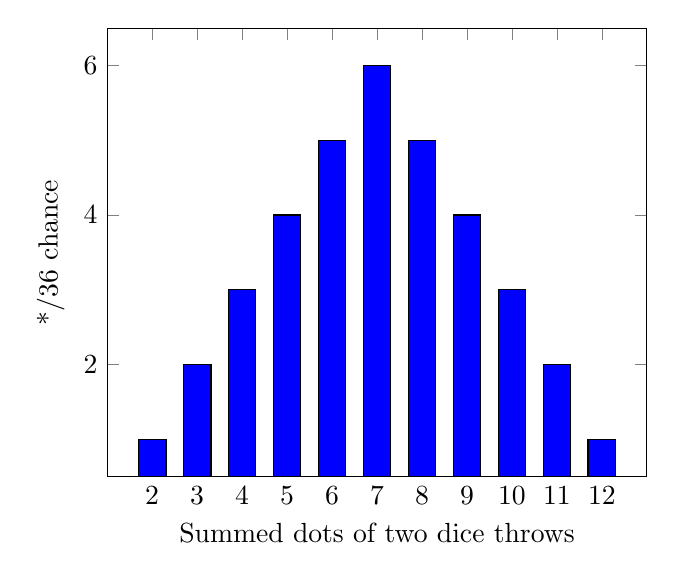
\begin{tikzpicture}
                    \begin{axis}[symbolic x coords={2,3,4,5,6,7,8,9,10,11,12},
                        xtick=data,
                        ylabel=*/36 chance,
                        xlabel=Summed dots of two dice throws
                      ]
                        \addplot[ybar,fill=blue] coordinates {
                            (2,  1)
                            (3,  2)
                            (4,  3)
                            (5,  4)
                            (6,  5)
                            (7,  6)
                            (8,  5)
                            (9,  4)
                            (10, 3)
                            (11, 2)
                            (12, 1)
                        };
                    \end{axis}
                \end{tikzpicture}

                
            \item
            	Laat $U$ wederom bestaan uit de opgetelde ogen 2 t/m 12.\\
            	Dan is de kans:
            		$$P(X=n) : n \in (2,3,4,5,6,7,8,9,10,11,12)$$
            \item
            	Met 2 dobbelstenen kan even ogen gegooid worden door met allebei
                de dobbelstenen even te gooien of door allebei met de
                dobbelstenen oneven te gooien, omdat er 1/2 kans is met iedere
                dobbelsteen even of oneven te gooien heb je 1/2 kans om even te
                gooien met 2 dobbelstenen.
        \end{enumerate}
       	\newpage

    \item
    	$$P(A \wedge B) = 0.4$$
    	$$P(A/B) = 0.1$$
    	$$P(B/A) = 0.3$$
    	$$P((B \vee A)^c) = 0.2$$

	\item
    	\begin{enumerate}
    		\item
    			$$
                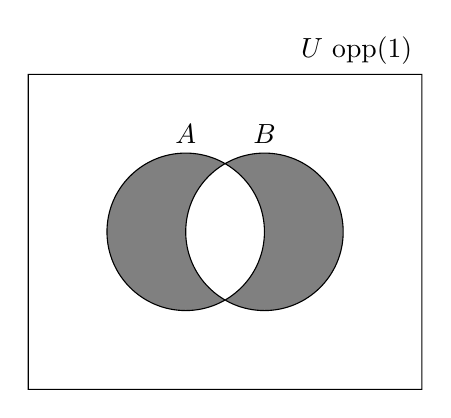
\begin{tikzpicture}[fill=gray]
                % left hand
                \scope
                \clip (-2,-2) rectangle (2,2)
                      (1,0) circle (1);
                \fill (0,0) circle (1);
                \endscope
                % right hand
                \scope
                \clip (-2,-2) rectangle (2,2)
                      (0,0) circle (1);
                \fill (1,0) circle (1);
                \endscope
                % outline
                \draw (0,0) circle (1) (0,1)  node [text=black,above] {$A$}
                      (1,0) circle (1) (1,1)  node [text=black,above] {$B$}
                      (-2,-2) rectangle (3,2) node [text=black,above left] {$U$ opp(1)};
                \end{tikzpicture}
				$$
                Intuitief is het goed te zien dat de kans op $A$ vereenigd $B$ in U de
                kans op A plus de kans op B is min de overlappende regio.
                In het geval van $A$ onafhankelijk $B$ is de overlappende regio
                nul, er zal van de optelling niks worden afgetrokken.
    			$$P(A \vee B) = P(A) + P(B) - P(A \wedge B)$$
    			$$P(A \vee B) = P(A) + P(B) - (P(A) + P(B) - P(A \vee B))$$
    			$$P(A \vee B) = P(A \vee B)$$
    			\\
    			$$P(A \vee B) = P(A) + P(B) - P(A \wedge B)$$
    			$$P(A \wedge \neg B) + P(A \wedge B) + P(\neg A \wedge B) = P(A) + P(B) - P(A \wedge B)$$
    			$$P(A) + P(\neg A \wedge B) = P(A) + P(B) - P(A \wedge B)$$
    			$$P(A) + P(B) - P(A \wedge B) = P(A) + P(B) - P(A \wedge B)$$
    		\item
    			$$P(\neg A) = 1 - P(A)$$
    			$$P(\neg A) + P(A) = 1$$
    			$$P(U) = 1$$

    		\item
                $$P(A) = P(A \wedge B) + P(A \wedge \neg B)$$
                $$P(A) = P(A \wedge (B \vee \neg B))$$
                $$P(A) = P(A \wedge U)$$
                $$P(A) = P(A)$$

            \item
                $$P(A) = \sum\limits_{i=1}^{n} P(A \wedge B_{i})$$
                $$P(A) = P(A \wedge \sum\limits_{i=1}^{n} B_{i})$$
                $$P(A) = P(A \wedge U)$$
                $$P(A) = P(A)$$

    	\end{enumerate}
    \item
    	$$P(A|B) = \frac{P(A)}{P(B)} P(B|A)$$
        $$P(A|B) = \frac{P(A)}{P(B)} \frac{P(B \wedge A)}{P(A)}$$
        $$P(A|B) = \frac{P(A) * P(B \wedge A)}{P(A) * P(B)}$$
        $$P(A|B) = \frac{\hcancel{P(A)}{0pt}{0pt}{0pt}{0pt} * P(B \wedge A)}{\hcancel{P(A)}{0pt}{0pt}{0pt}{0pt} * P(B)}$$
        $$P(A|B) = \frac{P(A \wedge B)}{P(B)}$$
        $$P(A|B) = P(A|B)$$
    \item
        \begin{enumerate}
            \item
    	       $$
                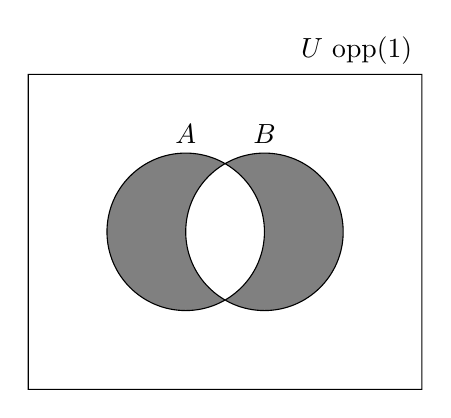
\begin{tikzpicture}[fill=gray]
                % left hand
                \scope
                \clip (-2,-2) rectangle (2,2)
                      (1,0) circle (1);
                \fill (0,0) circle (1);
                \endscope
                % right hand
                \scope
                \clip (-2,-2) rectangle (2,2)
                      (0,0) circle (1);
                \fill (1,0) circle (1);
                \endscope
                % outline
                \draw (0,0) circle (1) (0,1)  node [text=black,above] {$A$}
                      (1,0) circle (1) (1,1)  node [text=black,above] {$B$}
                      (-2,-2) rectangle (3,2) node [text=black,above left] {$U$ opp(1)};
                \end{tikzpicture}
				$$
            \item
                Het is goed te zien dat als aan B voldaan is dat de doorsnede
                van A en B de resterende invloed van A is in het nieuwe
                universum U = B. Omdat universum U nu B is moet er
                genormaliseerd worden naar B dus wordt er door de kans op
                B gedeeld.
        \end{enumerate}
    \item
        \begin{enumerate}
            \item
                $$P(A_{n-1}|A_n) = \frac{P(A_{n-1}A_n)}{P(A_n)}$$
                $$P(A_{n-1}A_n) = P(A_{n-1}|A_n)P(A_n) = X$$
                $$P(A_{n-2}|X) = \frac{P(A_{n-2}X)}{P(X)}$$
                $$P(A_{n-2}X) = P(A_{n-2}|X)P(X)$$
                $$P(A_n A_{n-1} A_{n-2}) = P(A_{n-2}|A_{n-1}A_n)P(A_{n-1}|A_n)P(A_n)$$
                $$herhaal$$
            \item
                De volgorde maakt niet uit.
        \end{enumerate}

    \item
        \begin{enumerate}
        \item
            \Tree[.U [.{vaas1 1/3} [[.{wit 5/6} \textit{5/18} ]
                                    [.{rood 1/6} \textit{1/18} ]]]
                    [.{vaas2 1/3} [[.{wit 2/3} \textit{2/9} ]
                           [.{rood 1/3} \textit{1/9} ]]]
                    [.{vaas3 1/3} [[.{wit 1/2} \textit{1/6} ]
                           [.{rood 1/2} \textit{1/6} ]]]
            ]

            $P(K=wit) = 5/18 + 2/9 + 1/6 = 12/18 = 2/3$
        \item
            $$P(A|B) = \frac{P(A \wedge B)}{P(B)}$$
        \end{enumerate}
    \item
        \begin{enumerate}
            \item
                $P(A \vee \neg B) \neq P(A)P(\neg B)$ tenzij $A = B$
            \item
                $P(\neg A \vee B) \neq P(\neg A)P(B)$ tenzij $A = B$
            \item
                $P(\neg A \vee \neg B) \neq P(\neg A)P(\neg B)$ tenzij $A \wedge B \neq 0$ en $A \vee B = U$
        \end{enumerate}        
    \item
        \Tree[.U [.{rood 1/3} [[.{vaas1 1/6} \textit{1/18} ][.{vaas2 1/3} \textit{1/9} ][.{vaas3 1/2} \textit{1/6} ]]]
                 [.{wit 2/3} [[.{vaas1 5/12} \textit{5/18} ][.{vaas2 1/3} \textit{2/9} ][.{vaas3 1/4} \textit{1/6} ]]]
             ]
\end{enumerate}

\end{document}
